\chapter{Studi Literatur}

\section{Jaringan Komputer}
Menurut \textcite{forouzan2012}, jaringan komputer merupakan sebuah keterhubungan dari beberapa perangkat yang dapat melakukan komunikasi satu sama lain. Perangkat yang dapat terlibat pada jaringan komputer ini sapat berupa \emph{host} seperti komputer, laptop, dan gawai lainnya. Selain itu, perangkat pada definisi di atas dapat berupa perangkat penghubung. Beberapa contoh dari perangkat penghubung adalah \emph{router}, \emph{switch}, dan \emph{modem}.

Terdapat empat buah syarat sebuah sistem dapat dikatakan sebagai jaringan komputer menurut \textcite{pratama2015}. Syarat-syarat yang perlu dipenuhi adalah sebagai berikut:
\begin{enumerate}
  \item Dalam sebuah sistem, setidaknya terdapat dua buah perangkat yang terhubung. Perangkat tersebut dapat terhubung melalui sarana kabel (\emph{wired}) ataupun sarana nirkabel (\emph{wireless}).
  \item Pada sistem ini, terdapat pengguna yang melakukan interaksi dengan pengguna lainnya. Pengguna ini dapat berupa penyedia layanan atau seseorang yang hendak melakukan komunikasi melewati jaringan komputer.
  \item Pada sistem ini, terdapat data yang dipertukarkan di dalamnya. Jenis data yang dipertukarkan dapat berupa pesan teks ataupun pesan biner.
  \item Terdapat sebuah sumber daya yang digunakan secara bersama-sama. Sumber daya ini dapat berupa perangkat keras ataupun perangkat lunak.
\end{enumerate}

\subsection{Pemodelan Jaringan TCP/IP}
Menurut \textcite{odom2022}, pemodelan jaringan merupakan kumpulan dari berbagai dokumen yang menjelaskan sebuah fungsionalitas dalam sebuah jaringan. Dokumen-dokumen ini akan mendefinisikan hal-hal yang terjadi pada jaringan komputer saat bekerja. Beberapa dokumen bisa saja menjelaskan sebuah protokol jaringan, yaitu kumpulan aturan yang perlu dipenuhi saat sebuah perangkat melakukan komunikasi pada jaringan komputer.

Pemodelan jaringan TCP/IP merupakan pemodelan terbaru yang memperbaiki kekurangan yang ada pada pemodelan \emph{layer} OSI (\cite{forouzan2012}). Selain itu, munculnya pemodelan jaringan TCP/IP dikarenakan pemodelan OSI \emph{layer} sudah tidak relevan dalam pemodelan jaringan. Faktanya, Pemodelan jaringan OSI pada saat ini sudah tidak ada lagi (\cite{odom2022}), tetapi beberapa protokol pada pemodelan TCP/IP masih merujuk pada protokol asli yang ada pada \emph{layer} OSI.

Pemodelan jaringan TCP/IP dibagi menjadi lima lapisan. Menurut \textcite{forouzan2012}, lapisan tersebut di antaranya sebagai berikut:

\begin{enumerate}
  \item \emph{Application Layer}: Lapisan ini menjelaskan spesifikasi aplikasi agar dapat berkomunikasi dalam jaringan komputer. Lapisan ini berfungsi sebagai antar muka antara aplikasi dengan jaringan. Beberapa contoh protokol yang berada pada lapisan ini adalah HTTP, FTP, dan SSH.
  \item \emph{Transport Layer}: Lapisan ini menjelaskan cara untuk memecah paket data menjadi unit-unit data yang lebih kecil (yang disebut sebagai \emph{segment}). Selain itu, lapisan ini juga berfungsi untuk memberikan penomoran setiap unit paket data sehingga data yang didapatkan akan terurut saat diberikan kepada aplikasi. Beberapa contoh protokol yang bekerja pada tingkatan ini adalah TCP dan UDP.
  \item \emph{Network Layer}: Lapisan ini menjelaskan bagaimana sebuah paket data dalam melakukan proses \emph{routing} untuk mencapai tujuan. Pada lapisan ini, dikenal sebuah sistem pengalamatan yang disebut dengan IP (\emph{Internet Protocol}) yang terstandarisasi secara internasional.
  \item \emph{Data Link Layer}: Lapisan ini bertugas untuk mengkontrol data, mengontrol kesalahan pada data saat pengiriman, serta pengalamatan fisik. Pada lapisan ini juga, didefinisikan cara untuk mengontrol aliran paket (\emph{Flow Control}) pada sebuah jaringan.
  \item \emph{Physical Layer}: Lapisan ini bertugas untuk menjelaskan perangkat keras dari sebuah jaringan komputer. Selain itu, lapisna ini juga bertugas untuk membantu proses persinyalan dan sinkronisasi bit data.
\end{enumerate}

\subsection{Protokol TCP}
Menurut \textcite{pratama2015}, Protokol TCP merupakan protokol jaringan pada lapisan \emph{transport} yang bersifat dapat diandalkan (\emph{reliable}) dan berbasis koneksi (\emph{connection oriented}). TCP memiliki sifat keandalan dikarenakan adanya proses pemeriksaan \emph{segment} yang dikirimkan ke komputer tujuan. Hal ini terlihat adanya pesan berupa konfirmasi dari penerima. Selain itu, TCP merupakan protokol berbasis koneksi. Hal ini dikarenakan saat sebelum melakukan pengiriman data, protokol ini mengharuskan untuk membentuk koneksi jaringan komputer terlebih dahulu. 

Menurut \textcite{peterson2011}, Terdapat beberapa layanan yang disediakan oleh protokol TCP. Layanan-layanan tersebut memberikan jaminan pada aplikasi bahwa data yang diterima dapat dipastikan terurut dan tidak hilang. Beberapa layanan yang disediakan di antaranya adalah sebagai berikut.

% Semuanya dari peterson2011 %
\begin{enumerate}
  \item Keandalan (\emph{Reliability}): Pada protokol TCP, data yang dikirimkan terjamin keterurutan saat diterima oleh penerima. Selain itu, proses pengiriman pada TCP bersifat \emph{full-duplex}. Hal ini berarti proses pengiriman data dapat dilakukan dua arah secara bersama-sama. Pada protokol ini juga, terdapat mekanisme kontrol aliran data. Hal ini memungkinkan untuk pengirim atau penerima menentukan jumlah data yang dikirimkan dalam satu waktu.
  \item Berbasis koneksi (\emph{Connection Oriented}): Protokol TCP mengharuskan pembuatan koneksi pada saat sebelum pengiriman data. Proses pembentukan koneksi ini perlu untuk membangun koneksi tidak hanya pada pengirim dan penerima, tetapi juga pada seluruh perangkat jaringan yang terlibat. Selain itu, protokol TCP juga mengharuskan pemutusan koneksi saat komunikasi berakhir. 
  \item Layanan pengiriman alir: Pada TCP, aplikasi memungkinkan untuk mengirimkan \emph{byte-byte} data menuju aliran jaringan. TCP akan menentukan seberapa banyak data yang akan dikirimkan menuju penerima.
\end{enumerate}

Menurut \textcite{pratama2015}, terdapat tiga tahap koneksi yang perlu dilakukan saat mengirimkan data. Ketiga tahap tersebut adalah pembentukan koneksi, pengiriman data, serta terminasi koneksi. Ketiga tahap ini perlu dilakukan dikarenakan sifat dari protokol TCP yaitu berbasiskan koneksi.

Tahap pertama yang perlu dilakukan dalam mengirim data melalui TCP adalah pembentukan koneksi. Proses pembentukan koneksi dilakukan dengan menggunakan \emph{three way handshake}. Menurut \textcite{peterson2011}, \emph{server} membentuk koneksi pasif dengan \emph{client}. Selanjutnya, \emph{client} mengirimkan \emph{segment} ACK menuju server. Setelah server menerima \emph{segment} ACK, server akan mengirimkan \emph{segment} SYN+ACK. Setelah itu, \emph{client} mengirimkan \emph{segment} ACK menuju \emph{server}. Setelah semua proses ini terjadi, koneksi antar \emph{client} dan \emph{server} telah terjalin. Proses ini dapat digambarkan pada \ref{fig:tcp.open}. 

\begin{figure}[!h]
  \centering
  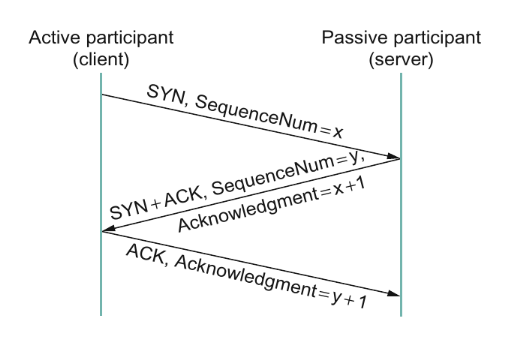
\includegraphics[width=280px]{chapters/res/chapter-2/img/tcp.open.png}
  \caption{Proses Pembukaan Koneksi TCP} \label{fig:tcp.open}
  Sumber: \textcite{peterson2011}
\end{figure}

Saat koneksi telah terjalin, pengiriman data sudah dapat dilakukan. Proses transfer data dilakukan dengan mengirimkan \emph{segment} data menuju penerima. Saat menerima data, penerima harus mengirimkan \emph{segment} ACK menuju pengirim. Apabila terjadi kegagalan transmisi, setiap \emph{segment} yang hilang harus ditransmisikan ulang.

Menurut \textcite{peterson2011}, setiap \emph{segment} yang dikirimkan diharapkan selalu penuh. Hal ini mencegah terjadi permasalahan \emph{silly window syndrome}. Oleh karena itu, pengiriman dapat diatur oleh algoritma nagle. Terdapat sebuah parameter untuk menentukan besar maksimum data yang dikirimkan yaitu nilai \emph{maximum segment size} (MSS).

Pada saat pengiriman data, terdapat juga sebuah nilai $Timeout$ yang menentukan apakah proses pengiriman \emph{segment} perlu diulang. Nilai ini dapat diturunkan melalui nilai estimasi \emph{round time trip} (RTT) dari sebuah data. Saat mengirimkan data, pengirim perlu menunggu ACK hingga batas $timeout$. Apabila telah terjadi timeout, pengirim perlu mengirimkan ulang data mereka menuju penerima. Semua proses pada tahap pengiriman ini perlu dilakukan hingga semua data berhasil dikirimkan.

Pada fase terakhir, koneksi antara \emph{client} dan \emph{server} perlu ditutup. Hal ini perlu dilakukan dengan \emph{client} melakukan proses \emph{active close}. Pada tahap \emph{active close}, \emph{client} mengirimkan pesan FIN. Setelah itu, \emph{server} mengirimkan pesan FIN+ACK. Setelah menerima pesan dari \emph{server}, \emph{client} perlu mengirimkan ACK. Setelah itu, koneksi antara \emph{server} dan \emph{client} telah tertutup.

\section{Kriptografi}
Menurut \textcite{schneier1996}, Kriptografi merupakan ilmu pengetahuan dan seni yang berujuan untuk menjaga sebuah pesan tetap aman. Menurut \textcite{anderson2008}, Kriptografi dianggap sebagai pintu para pengembang keamanan untuk bertemu dengan ilmu matematika. Hal ini dapat terlihat bahwa banyak sekali algoritma kriptografi yang terkait dengan konsep matematika. Kriptografi dianggap juga sebagai seni. Menurut \textcite{munir2019}, hal ini dikarenakan dari pandangan sejarah berkembangnya kriptografi. Kriptografi ini terbentuk dikarenakan adanya keinginan untuk merahasiakan sebuah pesan. Tentu saja, setiap orang memiliki ciri khas serta caranya tersendiri untuk menyandikan sebuah pesan. Oleh karena itu, kriptografi dapat dianggap sebagai seni untuk merahasiakan sebuah pesan. 

Kriptografi pada dasarnya memiliki beberapa layanan dasar yang dapat digunakan dalam dunia keamanan. Menurut \textcite{schneier1996}, beberapa layanan yang terdapat pada kriptografi adalah sebagai berikut:
\begin{enumerate}
  \item Kerahasiaan (\emph{confidentiality}) merupakan sebuah layanan yang diberikan oleh kriptografi untuk menjaga pesan agar pesan hanya dapat dimengerti oleh pihak yang memiliki otoritas. 
  \item Integritas (\emph{integrity}) merupakan layanan yang menjamin bahwa pesan yang diterima merupakan pesan yang belum pernah dilakukan modifikasi sebelumnya. Layanan ini menjamin data yang diterima sama dengan data tersebut saat pertama kali dikirim.
  \item Otentikasi (\emph{authentication}) merupakan layanan yang menjamin bahwa pesan yang diterima merupakan pesan yang dikirim oleh pengirim sesungguhnya. Hal ini terkait dengan klaim bahwa pesan yang dikirimkan tentu saja dapat dilakukan dekripsi dengan kunci yang telah disepakati.
  \item Anti penyangkalan (\emph{non-repudiation}) merupakan layanan yang menjamin bahwa pengirim tentu saja tidak akan dapat menyangkal pesan yang telah dia kirimkan.
\end{enumerate} 

Kriptografi modern, menurut \textcite{munir2019}, merupakan kriptografi yang bekerja pada komputer digital. Pesan tidak hanya terbatas pada tulisan dan alfabet, namun pesan juga dapat berupa berbentuk apapun selama dapat diubah menjadi bentuk biner. Dalam Kriptografi modern, terdapat sebuah konsep yang disebut dengan kriptografi kunci publik, konsep fungsi \emph{hash}, serta tanda tangan digital. Hal ini merupakan konsep baru yang dapat digunakan untuk menjamin integritas serta anti penyangkalan dari pengirim pesan.

Menurut \textcite{schneier1996}, keamanan kriptografi modern tidak hanya cukup apabila merahasiakan algoritma penguncian. Hal ini dikarenakan apabila sebuah algoritma penguncian dapat dipecahkan, algoritma tersebut perlu diganti dengan yang baru. Dalam kriptografi modern, kerahasiaan yang perlu dijaga terletak pada kunci. Setiap operasi enkripsi serta dekripsi tentu saja akan melibatkan kunci ini. 

Sebuah algoritma kriptografi tentu membutuhkan kunci untuk melakukan proses enkripsi dan dekripsi. Menurut \textcite{schneier1996}, algoritma kriptografi dapat dibagi menjadi dua, yaitu Kriptografi kunci simetrik dan kriptografi publik. Perbedaan dari kedua algoritma tersebut terletak pada kunci yang digunakan untuk melakukan enkripsi serta dekripsi pesan. 

Menurut \textcite{munir2019}, algoritma kunci simetri menggunakan kunci yang sama saat melakukan proses enkripsi serta dekripsi pesan. Asumsi yang diterapkan pada penggunaan algoritma ini adalah pengirim serta penerima sudah melakukan proses pembagian kunci. Skema proses enkripsi digambarkan pada gambar \ref{fig:crypto.symetric}.

\begin{figure}[!h]
  \centering
  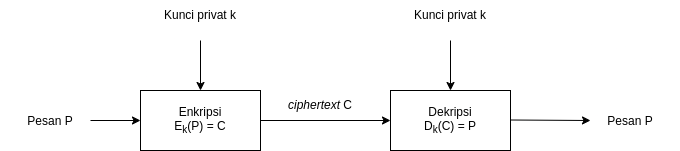
\includegraphics[width=\textwidth]{chapters/res/chapter-2/img/crypto.symetric.png}
  \caption{Visualisasi Proses Enkripsi Kriptografi Kunci Simetri} \label{fig:crypto.symetric}
  Sumber: \textcite{munir2019}
\end{figure}

Menurut \textcite{munir2019}, algoritma kriptografi kunci simetris ini dibagi lagi menjadi dua buah jenis, yaitu \emph{cipher} blok dan \emph{cipher} alir. Perbedaan antara kedua jenis \emph{cipher} tersebut terletak pada cara pengenkripsian sebuah pesan. Pada \emph{cipher} alir, proses enkripsi dilakukan dengan cara mengenkripsikan pesan per bit per bit. Proses penenkripsian juga tidak menutup kemungkinan dilakukan \emph{byte} per \emph{byte}. Contoh algoritma yang termasuk dalam \emph{cipher} alir adalah RC4 dan A5.

Menurut \textcite{munir2019}, Algoritma \emph{cipher} blok merupakan algoritma kunci simetris yang memproses pesan berdasarkan blok-blok bit atau \emph{byte}. Enkripsi dilakukan pada blok tersebut setiap kali. Terdapat beberapa operasi yang ada pada \emph{cipher} blok, di antaranya adalah ECB, CBC, CFB, dan OFB. Setiap operasi ini menentukan cara setiap blok pesan \emph{plaintext} atau \emph{ciphertext} dilakukan proses kriptografi.


\begin{figure}[!h]
  \centering
  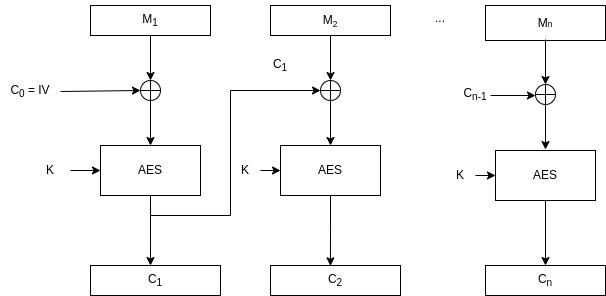
\includegraphics[width=\textwidth]{chapters/res/chapter-2/img/cbc.encrypt.png}
  \caption{Visualisasi Enkripsi Mode Blok CBC} 
  \label{fig:crypto.cbc.encrypt}
  Sumber: \textcite{munir2019}
\end{figure}


\begin{figure}[!h]
  \centering
  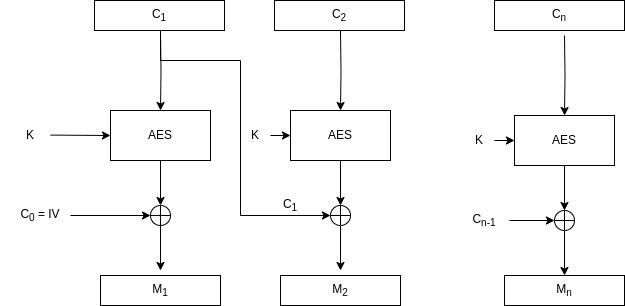
\includegraphics[width=\textwidth]{chapters/res/chapter-2/img/cbc.decrypt.png}
  \caption{Visualisasi Dekripsi Mode Blok CBC} 
  \label{fig:crypto.cbc.decrypt}
  Sumber: \textcite{munir2019}
\end{figure}

Salah satu bentuk mode blok yang sering digunakan dalam melakukan enkripsi adalah CBC. Menurut \textcite{munir2019}, mode enkripsi CBC menerapkan sistem enkripsi dengan cara memanfaatkan umpan balik dari hasil enkripsi blok sebelumnya. Nilai blok yang akan dienkripsi pertama-tama akan dilakukan XOR terlebih dahulu dengan umpan balik tersebut. Setelah itu, hasil XOR akan dienkripsi dengan kunci $K$. Nilai umpan balik awal disebut dengan $IV$. Nilai $IV$ tidak perlu dirahasiakan, tetapi perlu dibuat secara acak saat hendak melakukan proses enkripsi. Ilustrasi proses enkripsi menggunakan blok ini diilustrasikan pada figur \ref{fig:crypto.cbc.encrypt}, sedangkan ilustrasi proses dekripsi digambarkan pada figur \ref{fig:crypto.cbc.decrypt}. Secara matematis, proses ini ditunjukan pada persamaan \ref{eq:crypto.cbc.enc}.

\begin{equation}
  \label{eq:crypto.cbc.enc}
  \begin{array}{l}   
    Ct_i = E_K(P_i \oplus C_{i-1}) \\
    Pt_i = D_K(C_i) \oplus C_{i-1} \\
    C_0 = IV
  \end{array}
\end{equation}

Menurut \textcite{munir2019}, terdapat keuntungan saat menggunakan mode blok CBC dalam melakukan enkripsi. Keuntungan utamanya adalah hasil enkripsi akan memberikan hasil cipherteks yang berbeda untuk plainteks yang sama. Hal ini disebabkan adanya persebaran informasi antar tiap blok sehingga hasil enkripsi kedua blok tersebut dapat berbeda. Akan tetapi, kelemahan utama mode blok ini adalah perubahan satu bit pada cipherteks dapat membalikan satu bit pada blok setelahnya. Hal ini dapat digunakan pihak lawan untuk melakukan \emph{bit-flip attack} dengan memanfaatkan sifat ini. 

Menurut \textcite{munir2019}, algoritma kunci publik (atau bisa disebut algoritma kunci nirsimetris) merupakan algoritma enkripsi yang menggunakan kunci yang berbeda pada saat melakukan proses enkripsi dan juga proses dekripsi. Pada saat melakukan komunikasi menggunakan algoritma ini, pihak yang terlibat harus memiliki satu buah kunci, yaitu kunci publik dan kunci privat. Pengirim pesan akan menggunakan kunci publik untuk mengunci pesan. Akan tetapi, penerima menggunakan kunci privat miliknya untuk membuka pesan. Dengan menggunakan algoritma ini, hanya penerima pesan yang dapat membuka pesan. Ilustrasi terkait enkripsi memanfaatkan algoritma ini terdapat pada Gambar \ref{fig:crypto.asymetric}. Beberapa contoh algoritma enkripsi kunci publik adalah RSA, \emph{Elgamal}, dan DSA.

\begin{figure}[!h]
  \centering
  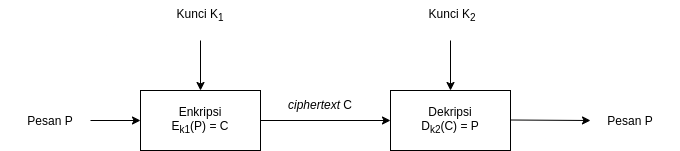
\includegraphics[width=\textwidth]{chapters/res/chapter-2/img/crypto.asymetric.png}
  \caption{Visualisasi Proses Enkripsi Kriptografi Kunci Publik} 
  \label{fig:crypto.asymetric}
  Sumber: \textcite{munir2019}
\end{figure}

Menurut \textcite{munir2019}, kriptografi kunci publik adadapat memberikan dua keuntungan. Keuntungan pertama adalah tidak adanya kebutuhan dalam mendistribusikan kunci rahasia. Kunci publik dapat dikirimkan melalui saluran yang tidak aman. Selain itu, keuntungan lain dari penggunaan kunci publik ini adalah jumlah pembuatan kunci dapat dikurangi. Pada saat menggunakan kriptografi kunci simetri, jumlah kunci yang harus dibuat adalah sebanyak jumlah pihak yang ingin berkomunikasi. Pada saat menggunakan algoritma asimetris, kunci yang perlu dibuat hanyalah sebanyak dua buah kunci, sehingga jumlah kunci menjadi lebih sedikit.

\section{Enkripsi Dinamis}
Enkripsi dinamis pertama kali dikenalkan oleh \textcite{knudsen2015}. Menurut \textcite{knudsen2015}, Enkripsi dinamis merupakan sebuah pendekatan kriptografi yang menyebabkan penerima pesan tidak perlu mengetahui detail proses enkripsi selain nilai dari \emph{secret key} dalam melakukan proses dekripsi. Pengirim pesan dapat menentukan algoritma enkripsi yang akan digunakan. Akan tetapi, penerima pesan tidak perlu mengetahui proses enkripsi yang dilakukan. Hal ini tentu mengharuskan bahwa penerima pesan dapat melakukan porses dekripsi dengan baik walaupun proses enkripsi tidak diketahui. 

Terdapat beberapa pendekatan yang ditawarkan oleh \textcite{knudsen2015}, salah satunya adalah dengan cara mengirimkan algoritma dekripsi $D$ ke penerima pesan. Pemilihan algoritma enkripsi dilakukan secara acak oleh pengirim. Pengiriman ini dilakukan dengan cara mengenkripsi algoritma $D$ dengan sistem enkripsi yang telah disepakati oleh kedua pihak. Penerima akan menjalankan algoritma dekripsi yang diterima untuk mendekripsi pesan. Berdasarkan \textcite{knudsen2015}, kelemahan dari pendekatan ini adalah transmisi kode \emph{executable}. Kode ini pun perlu dijalankan di penerima sehingga dapat membahayakan pengguna apabila kode yang dibuat merupakan kode yang berbahaya. Untuk mengatasi hal ini, diberikan beberapa solusi diantaranya adalah dengan memberikan pengecekan integritas dan otentikasi. Selain itu, perlu dilakukan juga pembatasan lingkungan eksekusi untuk melakukan proses dekripsi.

Menurut \textcite{knudsen2015}, terdapat varian lain dalam melakukan enkripsi dinamis, yaitu dengan menggunakan \emph{cipher} RAES. Pada \emph{cipher} RAES, proses enkripsi dilakukan sebagaimana AES-128 dilakukan. Akan tetapi, S-box yang digunakan berbeda. Terdapat dua buah kunci yang digunakan dalam melakukan enkripsi, yaitu kunci untuk digunakan pada AES-128 dan kunci untuk membangkitkan S-box. Menurut \textcite{knudsen2015}, keamanan menggunakan metode ini setidaknya sama kuatnya dengan menggunakan S-box.

\section{Pertukaran Kunci \emph{Diffie–Hellman}}
Algoritma pertukaran kunci \emph{Diffie–Hellman} merupakan algoritma yang digunakan untuk berbagi kunci sesi antara dua pihak atau lebih. Menurut \textcite{munir2019}, algoritma pertukaran kunci \emph{Diffie–Hellman} merupakan solusi dari permasalahan kriptografi kunci simetri, yaitu pengiriman kunci pada komunikasi jaringan yang tidak aman. Secara garis besar, setiap pihak yang akan melakukan pertukaran kunci menggunakan \emph{Diffie–Hellman}, akan mengirimkan parameter publiknya kepada setiap pihak. Penerima parameter publik akan membangkitkan kunci sesi berdasarkan parameter publik yang diterima dan parameter privat yang dimiliki olehnya. Ilustrasi pertukaran kunci ini digambarkan pada \ref{fig:crypto.dh}.

\begin{figure}[!h]
  \centering
  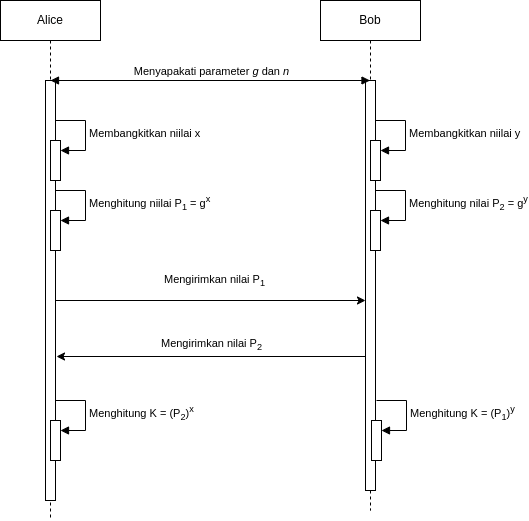
\includegraphics[width=\textwidth]{chapters/res/chapter-2/img/crypto.dh.png}
  \caption{Visualisasi Pertukaran Kunci \emph{Diffie-Hellman}} \label{fig:crypto.dh}
  Sumber: \textcite{munir2019}
\end{figure}

Pada ilustrasi yang ditunjukan \ref{fig:crypto.dh}, setiap pihak akan mendapatkan nilai $K$ yang sama. Nilai $K$ ini akan digunakan sebagai kunci sesi pada saat melakukan enkripsi menggunakan algoritma enkripsi kunci simetris.

Kekuatan dari pertukaran kunci \emph{Diffie–Hellman} menurut \textcite{munir2019} terletak pada sulitnya melakukan operasi logaritma diskrit. Nilai $x$ dan $y$ yang ditunjukan pada ilustrasi \ref{fig:crypto.dh} hanya dapat diekstrasi bila melakukan operasi logaritma diskrit dengan basis $g$. Menurut \textcite{staling2011}, Algoritma paling baik untuk mencari nilai logaritma diskrit saat ini berada pada kompleksitas $O(e^{(\ln{p})^{1/3} \cdot (\ln{(\ln{p})})^{2/3}})$ sehingga masih belum cukup mangkus untuk menyelesaikan persoalan ini untuk nilai $p$ yang besar.

\section{\emph{Advanced Encryption Standard (AES)}}
Menurut \textcite{staling2011}, Advanced Encryption Standard (AES) merupakan sebuah salah satu algoritma cipher blok yang dibuat dengan tujuan untuk menggantikan algoritma DES. Berdasarkan panjang kunci, algoritma AES dapat dibagi menjadi tiga, yaitu AES-128, AES-192, dan AES-256. Cipher AES akan melakukan enkripsi dan dekripsi dalam sejumlah \emph{round}. Jumlah \emph{round} yang akan dilakukan bergantung terhadap panjang kunci yang digunakan. Tabel \ref{tab:aes-round} menunjukan jumlah round yang digunakan pada spesifikasi algoritma AES.

\begin{longtable}{|c|c|}
  \caption{\label{tab:aes-round} Tabel Panjang Kunci dan Jumlah Round pada Algoritma AES} \\
  \hline
  Panjang Kunci & Jumlah Round \\ \hline
  128 bit       & 10           \\ \hline
  192 bit       & 12           \\ \hline
  256 bit       & 32           \\ \hline
\end{longtable}

Menurut \textcite{staling2011}, AES memiliki empat tahap yang digunakan dalam melakukan proses enkripsi. Tahap-tahap yang dilakukan dalam algoritma \emph{Rijndael} diantaranya adalah sebagai berikut:

\begin{enumerate}
  \item Tahap \emph{AddRoundKey}\\Menurut \textcite{munir2019}, Nilai \emph{state} akan dilakukan operasi XOR terhadap \emph{round key} pada tahap ini. Nilai \emph{round key} akan dibangkitkan melalui aloritma ekspansi kunci sehingga setiap \emph{round} akan memiliki kunci yang berbeda-beda.  
  \item Tahap Transformasi \emph{ShiftRow}\\Menurut \textcite{munir2019}, Nilai \emph{state} akan dilakukan pergeseran baris matriks secara \emph{wrapping}. Operasi ini bertujuan untuk mengubah urutan dalam plainteks. Jumlah pergeseran yang dilakukan ditentukan dengan posisi elemen baris pada matriks \emph{state}.
  \item Tahap \emph{MixColumns}\\Menurut \textcite{munir2019}, tahap ini merupakan pengacakan yang dilakukan pada nilai \emph{state}. Pada tahap ini, nilai \emph{state} akan dikalikan dengan matriks tertentu. Operasi perkalian yang digunakan merupakan perkalian pada $GF(2^8)$, sedangkan operasi penjumlahan yang digunakan merupakan XOR.
  \item Tahap \emph{Subtitute Bytes}\\Menurut \textcite{munir2019}, tahap ini merupakan tahap substitusi berdasarkan sebuah tabel yang bernama S-Box. Pada tahap ini, nilai pada \emph{state} akan dipetakan nilainya berdasarkan S-box yang digunakan. AES hanya memiliki sebuah table S-box yang digunakan pada setiap putaran serta pembangkitan kunci.
\end{enumerate}

Secara garis besar, proses enkripsi melalui algoritma \emph{Rijndael} ini ditunjukan pada gambar \ref{fig:crypto.aes}.


\begin{figure}[!h]
  \centering
  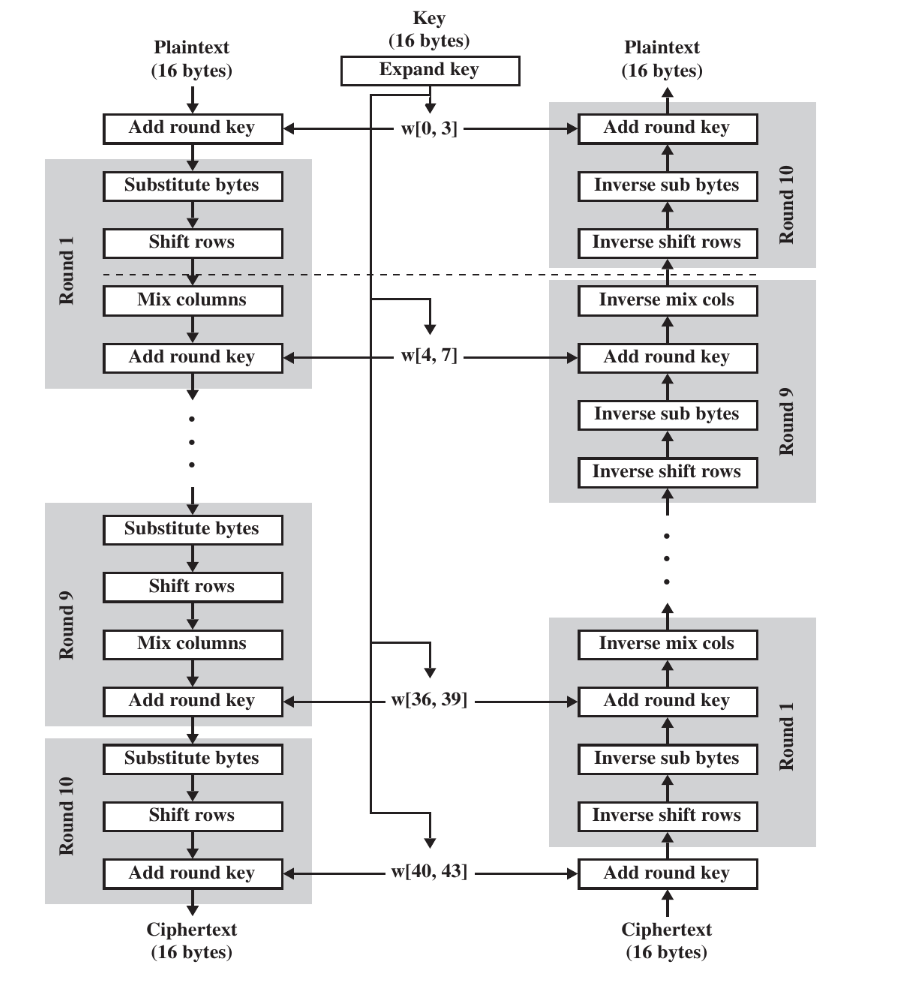
\includegraphics[width=\textwidth]{chapters/res/chapter-2/img/crypto.aes.png}
  \caption{Visualisasi Proses Enkripsi dan Dekripsi pada AES} \label{fig:crypto.aes}
  Sumber: \textcite{staling2011}\text

\end{figure}

\section{CSRPNG Berbasis \emph{Chaos}}
Menurut \textcite{munir2019}, Sistem chaos merupakan sistem matemtis yang dapat menghasilkan nilai dengan tidak teratur. Sistem chaos sangat peka terhadap perubahan kecil. Hal ini dikarenakan sistem chaos memiliki fenomena efek kupu-kupu.

Berdasarkan \textcite{boris2003}, terdapat tiga buah syarat sebuah sistem matematis dapat sebagai sistem chaos. Syarat tersebut diantaranya adalah sebagai berikut:
\begin{enumerate}
  \item Sistem tersebut haruslah sensitif terhadap nilai awal.
  \item Sistem tersebut harus memenuhi sifat \emph{topological transitive}. Hal ini berarti setiap nilai pada sistem chaos haruslah dapat dicapai dengan melakukan operasi sebuah fungsi secara berulang (\textcite{boris2003}).
  \item Sistem tersebut juga haruslah memiliki orbit periode yang padat.
\end{enumerate}

Menurut \textcite{munir2019}, Salah satu sifat yang dimiliki oleh sistem \emph{chaos} adalah ia bersifat deterministik. Selain itu, sistem chaos memiliki ketidakteraturan yang tinggi dalam menghasilkan nilai. SIfat yang paling penting adalah peka terhadap nilai awal. Semua sifat ini dapat memberikan sifat difusi pada algoritma kriptografi dikarenakan sistem chaos ini dapat menghilangkan hubungan statistik pada ciperteks.

Menurut \textcite{munir2019}, untuk membangkitkan nilai bilangan bulat, sistem \emph{chaos} haruslah dilakukan konversi menuju bilangan bulat. Salah satu fungsi yang dapat digunakan dalam melakukan konversi ini dinyatakan pada persamaan \ref{eq:chaos.linearization}.

\begin{equation}
  \label{eq:chaos.linearization}
  T(x, n) = \lfloor x \cdot 10^n \rfloor
\end{equation}

\section{Message Authentication Code (MAC)}
Menurut \textcite{munir2019}, Fungsi hash satu arah merupakan fungsi yang dapat menghasilkan sebuah \emph{message digest} yang tidak dapat dikembalikan menjadi pesan sesungguhnya. Dua pesan berbeda dapat menghasilkan nilai hash yang berbeda. Beberapa contoh fungsi hash adalah MD5 dan SHA-256.

Menurut \textcite{munir2019}, MAC merupakan perbaikan dari permasalahan yang muncul apabila menggunakan pengecekan integritas data memanfaatkan nilai hash. Dalam menjaga integritas sebuah data dengan menggunakan nilai hash saja, dapat menimbulkan kerentanan apabila data dan nilai hash diubah. MAC merupakan sebuah fungsi \emph{hash} satu arah yang menggunakan kunci rahasia dalam pembangkitannya.

\begin{figure}[!h]
  \centering
  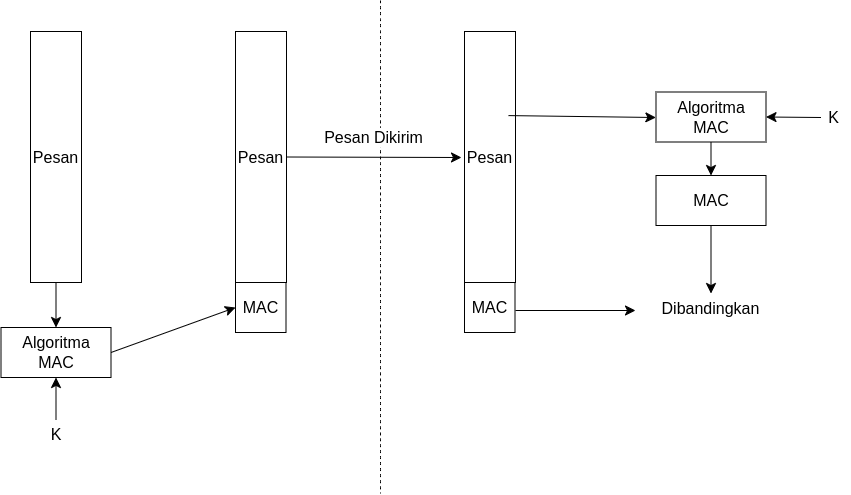
\includegraphics[width=350px]{chapters/res/chapter-2/img/mac.png}
  \caption{Ilustrasi proses pengiriman dan verifikasi pesan dengan MAC} \label{fig:mac}
  Sumber: \textcite{munir2019}
\end{figure}

Menurut \textcite{munir2019}, MAC dapat digunakan sebagai otentikasi pesan tanpa perlu melakukan enkripsi pada pesan tersebut. Hal ini dapat dilakukan dengan cara melekatkan nilai MAC pada pesan yang dikirimkan. Proses tersebut digambarkan pada figur \ref{fig:mac}. Proses verifikasi pesan dilakukan dengan membandingkan nilai MAC dari pesan yang dihitung ulang berdasarkan pesan yang diterima dengan nilai MAC yang dikirimkan. Apabila pesan tidak diubah, kedua nilai ini menghasilkan nilai yang sama. Keuntungan menggunakan MAC ini adalah adanya nilai $K$ sehingga nilai hash yang dilekatkan pada pesan tidak secara mudah dapat diganti.

\section{Penelitian Terkait}

Penelitian terkait enkripsi dinamis telah dilakukan oleh beberapa pihak. Berikut ini adalah beberapa penelitian yang berkaitan dengan enkripsi dinamis. 

\subsection{Sinkronisasi Kunci Dinamis berbasis Chaos den Aplikasinya pada Pengenkripsian Gambar dengan Algoritma AES yang diimprovisasi}

Menurut \textcite{lin2021}, kebutuhan keamanan data untuk berkomunikasi terus meningkat. Hal ini dikarenakan perkembangan sistem multimedia saat ini tentu terus berkembang. Salah satu variasi pengembangan algoritma enkripsi dan dekripsi yang berkembang saat ini menerapkan sinyal \emph{chaos}. 

Untuk memanfaatkan sistem \emph{chaos}, diperlukan sebuah parameter berupa nilai inisialisasi dari sistem chaos. Nilai ini perlu dipertukarkan melalui jaringan yang tidak aman, sehingga menambah peluang nilai tersebut dapat di-\emph{crack}. Terdapat beberapa pendekatan biasa dilakukan untuk mencapai sinkronisasi, yaitu menggunakan \emph{backstepping design}, \emph{fuzzy control}, dan \emph{sliding mode control}. Dari ketiga metode tersebut, mode yang sering digunakan adalah mode \emph{sliding mode control}. Penelitian yang dilakukan oleh (\cite{lin2021}) salah satunya akan berbicara terkait sinkronisasi sistem \emph{chaos} ini.

Penelitian ini juga termotivasi dengan adanya beberapa serangan yang biasa dilakukan oleh \emph{cracker} untuk memecahkan pesan \emph{ciphertext} memanfaatkan algoritma AES. Salah satu metode untuk melakukan serangan adalah memanfaatkan nilai \emph{cache}. Hal ini dapat terjadi dikarenakan pada saat ini, proses enkripsi menggunakan kunci simetri masih menggunakan kunci yang statis. Apabila kunci ini berhasil untuk dicuri, semua \emph{ciphertext} yang ada dapat dengan mudah untuk dilakukan dekripsi. Selain itu, perkembangan komputer kuantum juga menjadi tantangan tersendiri bagi AES. Komputer kuantum dapat memecahkan enkripsi AES dengan waktu yang cukup cepat. Oleh karena itu, penelitian ini juga terkait dengan modifikasi algoritma AES berbasis \emph{chaos} memanfaatkan kunci dinamis yang tersinkronisasi. Pengujian hasil dari algoritma AES berbasis \emph{chaos} ini dilakukan dengan cara melakukan enkripsi pada sebuah gambar. Analisis yang dilakukan diantaranya adalah analisis statis, histogram, entropi informasi, dan korelasi untuk menguji keamanan dan efisiensi dari algoritma yang telah dibentuk.

Pada penelitian \textcite{lin2021}, digunakan sistem \emph{chaos} berbasis Henon maps. Nilai \emph{chaos} ini dibagi menjadi dua buah bagian, yaitu \emph{master} dan \emph{slave}. Persamaan sistem \emph{chaos} untuk \emph{master} didefinisikan dengan persamaan \ref{eq:lin.henon.master}.

\begin{equation}
  \label{eq:lin.henon.master}
  \begin{array}{l}   
    x_1(k+1) = 1.76 - x_2^2(k) - 0.1 \cdot x_3(k)\\
    x_2(k+1) = x_1(k)\\
    x_3(k+1) = x_2(k)
  \end{array}
\end{equation}

Persamaan sistem \emph{chaos} untuk \emph{slave} didefinisikan dengan persamaan \ref{eq:lin.henon.slave}.

\begin{equation}
  \label{eq:lin.henon.slave}
  \begin{array}{l}   
    y_1(k+1) = 1.76 - x_2^2(k) - 0.1 \cdot x_3(k) + u(k)\\
    y_2(k+1) = y_1(k)\\
    y_3(k+1) = y_2(k)
  \end{array}
\end{equation}

Pada persamaan \ref{eq:lin.henon.slave}, nilai $u(k)$ merupakan nilai yang digunakan untuk melakukan proses sinkronisasi antara sistem \emph{chaos} yang dimiliki oleh \emph{master} dan \emph{slave}. Dari hasil penelitian tersebut, didefinisikan bahwa nilai sinkronisasi dapat dilakukan dengan persamaan berikut:

\begin{equation}
  \label{eq:lin.henon.sync}
  \begin{array}{l}   
    u(k) = \delta \cdot s(k) - [\alpha \cdot e_1(k) + (\beta - x_2(k) - y_2(k)) \cdot e_2(k) - 0.1 \cdot e_3(k)]\\
    s(k+1) = \delta \cdot s(k)
  \end{array}
\end{equation}

Nilai $|\delta|$ perlu kurang dari satu untuk mencapai sinkronisasi. Selain itu, Nilai $\alpha$ dan $\beta$ perlu dipilih sehingga semua nilai eigen matriks A yang didefinisikan pada persamaan \ref{eq:lin.henon.a-matrix} bernilai kurang dari 1. Niali $e_i(k)$ merupakan nilai error yang dihasilkan antara sistem slave dan sistem master. Oleh karena itu, nilai error tersebut didefinisikan dengan $e_i(k) = y_i(k) - x_i(k), i = 1,2,3$.

\begin{equation}
\label{eq:lin.henon.a-matrix}
A = \begin{bmatrix}
  -\alpha & -\beta \\
  1 & 0 
  \end{bmatrix}
\end{equation}

Dalam membangkitkan kunci dinamis, \textcite{lin2021} memanfaatkan fungsi hash SHA256. Hal ini bertujuan untuk memberikan panjang yang cukup pada saat melakukan enkripsi menggunakan AES. Ilustrasi dari proses pembangkitan kunci ini dapat dilihat pada gambar \ref{fig:lin.keygen}.

\begin{figure}[!h]
  \centering
  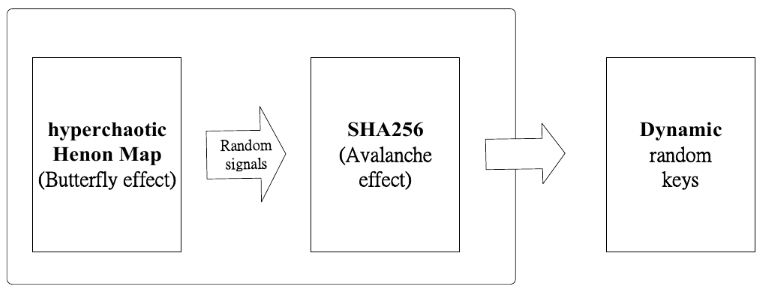
\includegraphics[width=350px]{chapters/res/chapter-2/img/lin.keygen.png}
  \caption{Ilustrasi proses pembangkitan kunci dinamis} \label{fig:lin.keygen}
  Sumber: \textcite{lin2021}
\end{figure}

Proses sinkronisasi sistem \emph{chaos} dapat dilakukan dengan mendekomposisi nilai $u(k)$ menjadi nilai $u_m(k)$ dan $u_s(k)$. Pemecahan nilai ini ditujukan untuk meningkatkan kemananan saat implementasi. Nilai $u_m(k)$ akan dikirimkan dari \emph{transmitter} menuju \emph{receiver}. Sistem ini dapat dijelaskan melalui gambar . Menurut \textcite{lin2021}, sistem itu aman. Hal ini dikarenakan apabla \emph{hacker} memiliki parameter-parameter yang digunakan untuk sinkronisasi, mereka tidak dapat mendapatkan \emph{state} dari master dan slave. Ilustrasi yang proses enkripsi dan dekripsi serta sinkronisasi yang dilakukan terdapat pada gambar \ref{fig:lin.caes}.

\begin{figure}[!h]
  \centering
  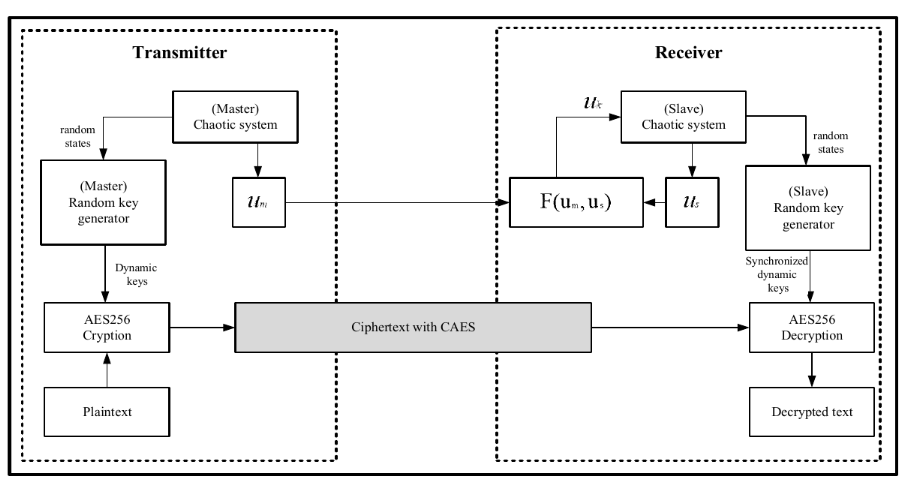
\includegraphics[width=350px]{chapters/res/chapter-2/img/lin.caes.png}
  \caption{Arsitektur AES berbasis \emph{chaos} yang telah diimporvisasi} \label{fig:lin.caes}
  Sumber: \textcite{lin2021}
\end{figure}

Pengujian dari sistem yang dilakukan oleh \textcite{lin2021} adalah dengan cara membandingkan proses enkripsi gambar yang dihasilkan memanfaatkan AES-ECB, AES-CBC, dan CAES-EBC. Gambar yang diuji merupakan gambar berukuran $256 \times 256$. Pada algoritma CAES, kunci dinamis yang dihasilkan sebanyak 49.152 kunci. Setiap kunci ini dibuat secara langsung melalui proses \emph{update} pada setiap \emph{round} enkripsi. Hasil enkripsi pada figur \ref{fig:lin.result} menunjukan bahwa CAES-ECB bila diobservasi secara visual memiliki kualitas yang cukup baik bila dibandingkan dengan AES-EBC. Menurut \textcite{lin2021}, Hal ini dapat membuktikan bahwa algoritma CAES-CBC lebih unggul dibandingkan AES-EBC dan AES-CBC.

\begin{figure}[!h]
  \centering
  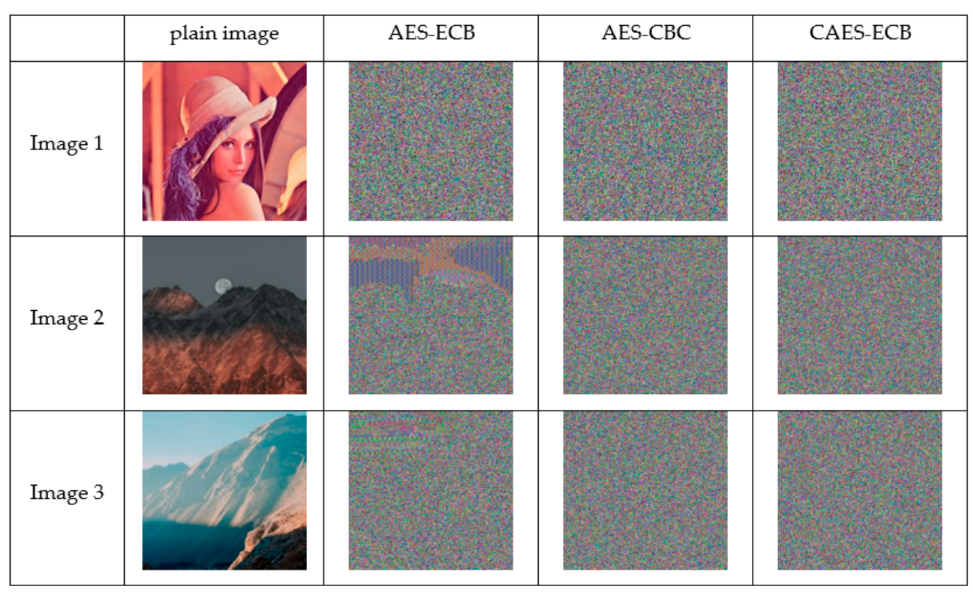
\includegraphics[width=350px]{chapters/res/chapter-2/img/lin.res.png}
  \caption{Hasil visual gambar terenkripsi} \label{fig:lin.result}
  Sumber: \textcite{lin2021}
\end{figure}

Proses enkripsi tersebut juga dilakukan proses pengujian secara analitik. Tes yang dilakukan berdasarkan parameter uji yang telah didefinisikan oleh National Institute of Standards and Technology (NIST). Pengujian yang dilakukan oleh \textcite{lin2021} menggunakan data \emph{stream} sepanjang 10.000.000 bit data dengan jumlah biat setiap stream sebesar 30. Hasil tersebut menunjukan bahwa algoritma CAES memenuhi persyaranan NIST SP 800-22 \emph{random number detection}. Hasil dari pengujian NIST juga menunjukan bahwa algoritma CAES lebih unggul dibandingkan dengan AES-CBC dan AES-EBC. Hal ini ditunjukan dengan data pada figur \ref{fig:lin.analytic-result}.

\begin{figure}[!h]
  \centering
  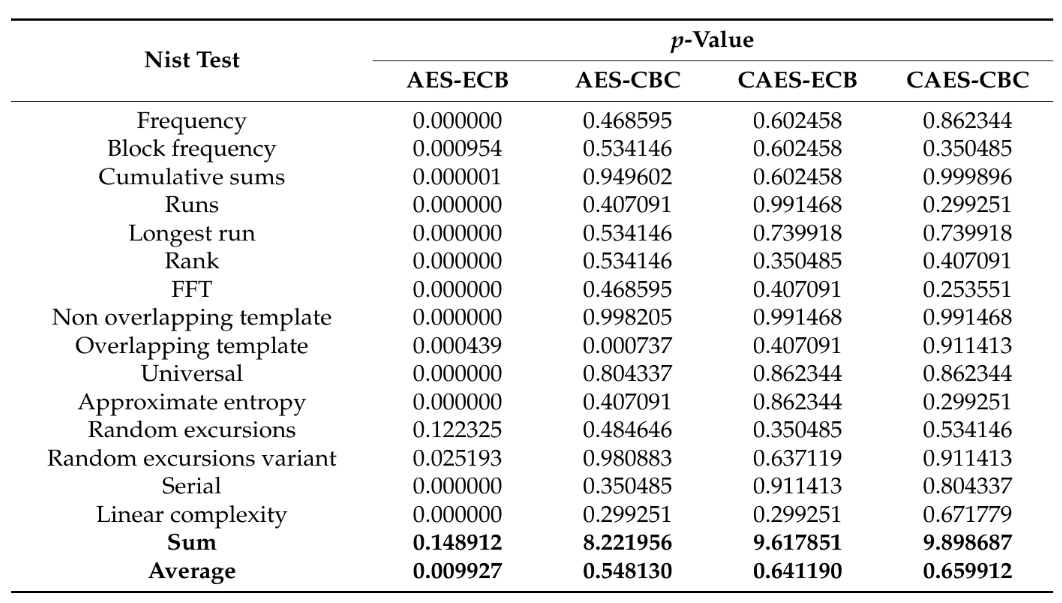
\includegraphics[width=350px]{chapters/res/chapter-2/img/lin.analytic-test.png}
  \caption{Hasil Analitik Algoritma CAES} \label{fig:lin.analytic-result}
  Sumber: \textcite{lin2021}
\end{figure}

\subsection{Enkripsi Gambar dan Analisisnya memanfaatkan Algoritma AES dinamis}

Pada penelitian yang dilakukan oleh \textcite{singh2019}, kedinamisan proses enkripsi dilakukan pada S-box. Pada penelitian ini, S-box yang dimiliki oleh AES akan dipermutasi. Terdapat tiga parameter yang digunakan dalam pembentukan S-box ini, yaitu sebagai berikut:
\begin{enumerate}
  \item Kunci\\ Kunci sangat berpengruh terhadap hasil S-box yang dibentuk. Perubahan kecil pada kunci perlu menyebabkan S-box keluaran yang jauh berbeda.
  \item \emph{Irreducible polynomial}\\ Pada penelitian yang dilakukan oleh \textcite{singh2019}, pemilihan \emph{Irreducible polynomial} dilakukan secara acak. Hal ini berbeda dengan algoritma AES pada umumnya yang hanya menggunakan satu polinomial yang digunakan untuk membentuk S-box.
  \item Konstanta Affine\\ Konstanta affine yang digunakan dalam pembentukan S-box. Terdapat 256 konstanta yang dapat digunakan. Dalam penelitian yang dilakukan \textcite{singh2019}, semua konstanta yang dapat digunakan dipilih secara acak untuk membentuk S-box.
\end{enumerate}

Menurut \textcite{singh2019}, S-box yang dapat dibentuk sangat sensitif terhadap tiga parameter diatas. Dengan menggunakan metode tersebut, jumlah kemungkinan S-box dinamis yang dapat dibentuk adalah $256!$. Hal ini dapat memberikan tambahan keamanan pada cipherteks dikarenakan kerumitan tidak hanya berada pada kunci tetapi terdapat pada algoritma.

Pada penelitian \textcite{singh2019}, algoritma enkripsi yang telah dijelaskan sebelumnya diuji dengan melakukan enkripsi gambar \emph{grayscale}. Pengujian yang dilakukan adalah pengujian analisis histogram, pengujian korelasi koefisien, kualitas enkripsi, entropi informasi, dan NPCR-UACI test. Hasil pengujian menunjukan bahwa AES dan Dynamic AES memiliki kualitas enkripsi yang cukup setara. Akan tetapi, dalam pengujian korelasi koefisien, AES dinamis memiliki hasil yang lebih baik dibandingkan dengan AES.

\subsection{Perbaikan Keamanan dari Algoritma AES memanfaatkan \emph{Salt} Dinamis}

Pada penelitian yang dilakukan oleh \textcite{bachtiar2018}, proses enkripsi dinamis dilakukan dengan cara menambahkan \emph{salt} pada pesan yang akan dienkripsi. Nilai \emph{salt} dibuat berdasarkan hasil dari algortima \emph{Linear Congruental Generator} (LCG). Secara global, proses enkripsi dilakukan dengan melakukan proses enkripsi dinamis terlebih dahulu. Setelah itu, proses enkripsi akan dilakukan dengan melakukan AES pada pesan yang telah dilakukan enkripsi dinamis. Proses ini dapat digambarkan pada figur \ref{fig:bachtiar.enc.process}.

\begin{figure}[!h]
  \centering
  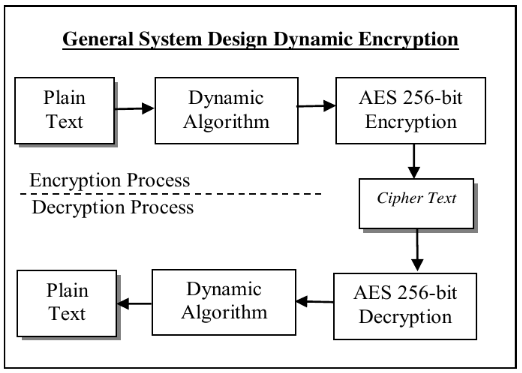
\includegraphics[width=250px]{chapters/res/chapter-2/img/bachtiar.enc.process.png}
  \caption{Ilustrasi proses pembangkitan kunci dinamis} \label{fig:bachtiar.enc.process}
  Sumber: \textcite{bachtiar2018}
\end{figure}

Pada proses enkripsi dinamis, akan dihitung \emph{salt} berdasarkan waktu. Nilai \emph{salt} akan dibuat melalui algoritma LCG.  Nilai salt ini akan ditambahkan pada pesan. Setelah pesan ditambahkan dengan \emph{salt}, pesan akan dilakukan proses enkripsi terlebih dahulu menggunakan OTP. Kunci yang digunakan untuk melakukan OTP merupakan kunci yang sama yang akan digunakan pada proses enkripsi menggunakan AES. Setelah proses ini dilakukan, pesan dinamis tersebut akan dienkripsi menggunakan AES.

Berdasarkan hasil pengujian yang dilakukan menggunakan NIST, teknik memanfaatkan pesan dinamis memberikan hasil yang lebih baik dibandingkan dengan tanpa menggunakan \emph{salt} atapun dengan hanya memanfaatkan \emph{salt} saja. Teknik memanfaatkan pesan dinamis untuk melakukan enkripsi secara dinamis memberikan nilai keberhasilan sebesar $72.5\%$. Nilai keberhasilan ini diperoleh berdasarkan pengujian dengan menjalankan sebanyak delapan kali dan dilakukan perhitungan secara rata-rata.
